\documentclass[]{article}
\usepackage{lmodern}
\usepackage{amssymb,amsmath}
\usepackage{ifxetex,ifluatex}
\usepackage{fixltx2e} % provides \textsubscript
\ifnum 0\ifxetex 1\fi\ifluatex 1\fi=0 % if pdftex
  \usepackage[T1]{fontenc}
  \usepackage[utf8]{inputenc}
\else % if luatex or xelatex
  \ifxetex
    \usepackage{mathspec}
  \else
    \usepackage{fontspec}
  \fi
  \defaultfontfeatures{Ligatures=TeX,Scale=MatchLowercase}
\fi
% use upquote if available, for straight quotes in verbatim environments
\IfFileExists{upquote.sty}{\usepackage{upquote}}{}
% use microtype if available
\IfFileExists{microtype.sty}{%
\usepackage{microtype}
\UseMicrotypeSet[protrusion]{basicmath} % disable protrusion for tt fonts
}{}
\usepackage[margin=1in]{geometry}
\usepackage{hyperref}
\hypersetup{unicode=true,
            pdftitle={DATA 608 - Project 1},
            pdfauthor={Joshua Sturm},
            pdfborder={0 0 0},
            breaklinks=true}
\urlstyle{same}  % don't use monospace font for urls
\usepackage{color}
\usepackage{fancyvrb}
\newcommand{\VerbBar}{|}
\newcommand{\VERB}{\Verb[commandchars=\\\{\}]}
\DefineVerbatimEnvironment{Highlighting}{Verbatim}{commandchars=\\\{\}}
% Add ',fontsize=\small' for more characters per line
\usepackage{framed}
\definecolor{shadecolor}{RGB}{248,248,248}
\newenvironment{Shaded}{\begin{snugshade}}{\end{snugshade}}
\newcommand{\KeywordTok}[1]{\textcolor[rgb]{0.13,0.29,0.53}{\textbf{#1}}}
\newcommand{\DataTypeTok}[1]{\textcolor[rgb]{0.13,0.29,0.53}{#1}}
\newcommand{\DecValTok}[1]{\textcolor[rgb]{0.00,0.00,0.81}{#1}}
\newcommand{\BaseNTok}[1]{\textcolor[rgb]{0.00,0.00,0.81}{#1}}
\newcommand{\FloatTok}[1]{\textcolor[rgb]{0.00,0.00,0.81}{#1}}
\newcommand{\ConstantTok}[1]{\textcolor[rgb]{0.00,0.00,0.00}{#1}}
\newcommand{\CharTok}[1]{\textcolor[rgb]{0.31,0.60,0.02}{#1}}
\newcommand{\SpecialCharTok}[1]{\textcolor[rgb]{0.00,0.00,0.00}{#1}}
\newcommand{\StringTok}[1]{\textcolor[rgb]{0.31,0.60,0.02}{#1}}
\newcommand{\VerbatimStringTok}[1]{\textcolor[rgb]{0.31,0.60,0.02}{#1}}
\newcommand{\SpecialStringTok}[1]{\textcolor[rgb]{0.31,0.60,0.02}{#1}}
\newcommand{\ImportTok}[1]{#1}
\newcommand{\CommentTok}[1]{\textcolor[rgb]{0.56,0.35,0.01}{\textit{#1}}}
\newcommand{\DocumentationTok}[1]{\textcolor[rgb]{0.56,0.35,0.01}{\textbf{\textit{#1}}}}
\newcommand{\AnnotationTok}[1]{\textcolor[rgb]{0.56,0.35,0.01}{\textbf{\textit{#1}}}}
\newcommand{\CommentVarTok}[1]{\textcolor[rgb]{0.56,0.35,0.01}{\textbf{\textit{#1}}}}
\newcommand{\OtherTok}[1]{\textcolor[rgb]{0.56,0.35,0.01}{#1}}
\newcommand{\FunctionTok}[1]{\textcolor[rgb]{0.00,0.00,0.00}{#1}}
\newcommand{\VariableTok}[1]{\textcolor[rgb]{0.00,0.00,0.00}{#1}}
\newcommand{\ControlFlowTok}[1]{\textcolor[rgb]{0.13,0.29,0.53}{\textbf{#1}}}
\newcommand{\OperatorTok}[1]{\textcolor[rgb]{0.81,0.36,0.00}{\textbf{#1}}}
\newcommand{\BuiltInTok}[1]{#1}
\newcommand{\ExtensionTok}[1]{#1}
\newcommand{\PreprocessorTok}[1]{\textcolor[rgb]{0.56,0.35,0.01}{\textit{#1}}}
\newcommand{\AttributeTok}[1]{\textcolor[rgb]{0.77,0.63,0.00}{#1}}
\newcommand{\RegionMarkerTok}[1]{#1}
\newcommand{\InformationTok}[1]{\textcolor[rgb]{0.56,0.35,0.01}{\textbf{\textit{#1}}}}
\newcommand{\WarningTok}[1]{\textcolor[rgb]{0.56,0.35,0.01}{\textbf{\textit{#1}}}}
\newcommand{\AlertTok}[1]{\textcolor[rgb]{0.94,0.16,0.16}{#1}}
\newcommand{\ErrorTok}[1]{\textcolor[rgb]{0.64,0.00,0.00}{\textbf{#1}}}
\newcommand{\NormalTok}[1]{#1}
\usepackage{graphicx,grffile}
\makeatletter
\def\maxwidth{\ifdim\Gin@nat@width>\linewidth\linewidth\else\Gin@nat@width\fi}
\def\maxheight{\ifdim\Gin@nat@height>\textheight\textheight\else\Gin@nat@height\fi}
\makeatother
% Scale images if necessary, so that they will not overflow the page
% margins by default, and it is still possible to overwrite the defaults
% using explicit options in \includegraphics[width, height, ...]{}
\setkeys{Gin}{width=\maxwidth,height=\maxheight,keepaspectratio}
\IfFileExists{parskip.sty}{%
\usepackage{parskip}
}{% else
\setlength{\parindent}{0pt}
\setlength{\parskip}{6pt plus 2pt minus 1pt}
}
\setlength{\emergencystretch}{3em}  % prevent overfull lines
\providecommand{\tightlist}{%
  \setlength{\itemsep}{0pt}\setlength{\parskip}{0pt}}
\setcounter{secnumdepth}{0}
% Redefines (sub)paragraphs to behave more like sections
\ifx\paragraph\undefined\else
\let\oldparagraph\paragraph
\renewcommand{\paragraph}[1]{\oldparagraph{#1}\mbox{}}
\fi
\ifx\subparagraph\undefined\else
\let\oldsubparagraph\subparagraph
\renewcommand{\subparagraph}[1]{\oldsubparagraph{#1}\mbox{}}
\fi

%%% Use protect on footnotes to avoid problems with footnotes in titles
\let\rmarkdownfootnote\footnote%
\def\footnote{\protect\rmarkdownfootnote}

%%% Change title format to be more compact
\usepackage{titling}

% Create subtitle command for use in maketitle
\newcommand{\subtitle}[1]{
  \posttitle{
    \begin{center}\large#1\end{center}
    }
}

\setlength{\droptitle}{-2em}
  \title{DATA 608 - Project 1}
  \pretitle{\vspace{\droptitle}\centering\huge}
  \posttitle{\par}
  \author{Joshua Sturm}
  \preauthor{\centering\large\emph}
  \postauthor{\par}
  \predate{\centering\large\emph}
  \postdate{\par}
  \date{02/08/2018}


\begin{document}
\maketitle

\begin{Shaded}
\begin{Highlighting}[]
\CommentTok{# Load packages}
\NormalTok{packages <-}\StringTok{ }\KeywordTok{c}\NormalTok{(}\StringTok{"tidyverse"}\NormalTok{)}
\KeywordTok{invisible}\NormalTok{(}\KeywordTok{lapply}\NormalTok{(packages, library, }\DataTypeTok{character.only =}\NormalTok{ T))}
\end{Highlighting}
\end{Shaded}

\textbf{Principles of Data Visualization and Introduction to ggplot2}

I have provided you with data about the 5,000 fastest growing companies
in the US, as compiled by Inc. magazine. lets read this in:

\begin{Shaded}
\begin{Highlighting}[]
\NormalTok{inc <-}\StringTok{ }\KeywordTok{read.csv}\NormalTok{(}\StringTok{"https://raw.githubusercontent.com/charleyferrari/CUNY_DATA_608/master/module1/Data/inc5000_data.csv"}\NormalTok{, }\DataTypeTok{header=} \OtherTok{TRUE}\NormalTok{)}
\end{Highlighting}
\end{Shaded}

And lets preview this data:

\begin{Shaded}
\begin{Highlighting}[]
\KeywordTok{head}\NormalTok{(inc)}
\end{Highlighting}
\end{Shaded}

\begin{verbatim}
##   Rank                         Name Growth_Rate   Revenue
## 1    1                         Fuhu      421.48 1.179e+08
## 2    2        FederalConference.com      248.31 4.960e+07
## 3    3                The HCI Group      245.45 2.550e+07
## 4    4                      Bridger      233.08 1.900e+09
## 5    5                       DataXu      213.37 8.700e+07
## 6    6 MileStone Community Builders      179.38 4.570e+07
##                       Industry Employees         City State
## 1 Consumer Products & Services       104   El Segundo    CA
## 2          Government Services        51     Dumfries    VA
## 3                       Health       132 Jacksonville    FL
## 4                       Energy        50      Addison    TX
## 5      Advertising & Marketing       220       Boston    MA
## 6                  Real Estate        63       Austin    TX
\end{verbatim}

\begin{Shaded}
\begin{Highlighting}[]
\KeywordTok{summary}\NormalTok{(inc)}
\end{Highlighting}
\end{Shaded}

\begin{verbatim}
##       Rank                          Name       Growth_Rate     
##  Min.   :   1   (Add)ventures         :   1   Min.   :  0.340  
##  1st Qu.:1252   @Properties           :   1   1st Qu.:  0.770  
##  Median :2502   1-Stop Translation USA:   1   Median :  1.420  
##  Mean   :2502   110 Consulting        :   1   Mean   :  4.612  
##  3rd Qu.:3751   11thStreetCoffee.com  :   1   3rd Qu.:  3.290  
##  Max.   :5000   123 Exteriors         :   1   Max.   :421.480  
##                 (Other)               :4995                    
##     Revenue                                  Industry      Employees      
##  Min.   :2.000e+06   IT Services                 : 733   Min.   :    1.0  
##  1st Qu.:5.100e+06   Business Products & Services: 482   1st Qu.:   25.0  
##  Median :1.090e+07   Advertising & Marketing     : 471   Median :   53.0  
##  Mean   :4.822e+07   Health                      : 355   Mean   :  232.7  
##  3rd Qu.:2.860e+07   Software                    : 342   3rd Qu.:  132.0  
##  Max.   :1.010e+10   Financial Services          : 260   Max.   :66803.0  
##                      (Other)                     :2358   NA's   :12       
##             City          State     
##  New York     : 160   CA     : 701  
##  Chicago      :  90   TX     : 387  
##  Austin       :  88   NY     : 311  
##  Houston      :  76   VA     : 283  
##  San Francisco:  75   FL     : 282  
##  Atlanta      :  74   IL     : 273  
##  (Other)      :4438   (Other):2764
\end{verbatim}

Think a bit on what these summaries mean. Use the space below to add
some more relevant non-visual exploratory information you think helps
you understand this data:

\begin{Shaded}
\begin{Highlighting}[]
\KeywordTok{glimpse}\NormalTok{(inc) }\CommentTok{# View number of rows and columns, variable types}
\end{Highlighting}
\end{Shaded}

\begin{verbatim}
## Observations: 5,001
## Variables: 8
## $ Rank        <int> 1, 2, 3, 4, 5, 6, 7, 8, 9, 10, 11, 12, 13, 14, 15,...
## $ Name        <fct> Fuhu, FederalConference.com, The HCI Group, Bridge...
## $ Growth_Rate <dbl> 421.48, 248.31, 245.45, 233.08, 213.37, 179.38, 17...
## $ Revenue     <dbl> 1.179e+08, 4.960e+07, 2.550e+07, 1.900e+09, 8.700e...
## $ Industry    <fct> Consumer Products & Services, Government Services,...
## $ Employees   <int> 104, 51, 132, 50, 220, 63, 27, 75, 97, 15, 149, 16...
## $ City        <fct> El Segundo, Dumfries, Jacksonville, Addison, Bosto...
## $ State       <fct> CA, VA, FL, TX, MA, TX, TN, CA, UT, RI, VA, CA, FL...
\end{verbatim}

\subsection{Question 1}\label{question-1}

Create a graph that shows the distribution of companies in the dataset
by State (ie how many are in each state). There are a lot of States, so
consider which axis you should use. This visualization is ultimately
going to be consumed on a `portrait' oriented screen (ie taller than
wide), which should further guide your layout choices.

\subsubsection{Since we'll be displaying the output on a portrait
screen, we want to flip the coordinates, and use the y
axis.}\label{since-well-be-displaying-the-output-on-a-portrait-screen-we-want-to-flip-the-coordinates-and-use-the-y-axis.}

\begin{Shaded}
\begin{Highlighting}[]
\CommentTok{# Group by state, and take the count}
\NormalTok{state.count <-}\StringTok{ }\NormalTok{inc }\OperatorTok
\StringTok{  }\KeywordTok{count}\NormalTok{(State)}

\KeywordTok{ggplot}\NormalTok{(state.count, }\KeywordTok{aes}\NormalTok{(}\DataTypeTok{x=}\KeywordTok{reorder}\NormalTok{(State, n), }\DataTypeTok{y=}\NormalTok{n)) }\OperatorTok{+}\StringTok{ }
\StringTok{  }\KeywordTok{geom_bar}\NormalTok{(}\DataTypeTok{stat=}\StringTok{"identity"}\NormalTok{, }\DataTypeTok{fill=}\StringTok{"firebrick2"}\NormalTok{, }\DataTypeTok{width=}\FloatTok{0.5}\NormalTok{) }\OperatorTok{+}\StringTok{ }
\StringTok{  }\KeywordTok{coord_flip}\NormalTok{() }\OperatorTok{+}
\StringTok{  }\KeywordTok{labs}\NormalTok{(}\DataTypeTok{title=}\StringTok{"Number of companies by State"}\NormalTok{, }
       \DataTypeTok{subtitle=}\StringTok{"count vs. State"}\NormalTok{,}
       \DataTypeTok{x =} \StringTok{"State"}\NormalTok{,}
       \DataTypeTok{y =} \StringTok{"Count"}\NormalTok{) }\OperatorTok{+}\StringTok{ }
\StringTok{  }\KeywordTok{theme_grey}\NormalTok{(}\DataTypeTok{base_size =} \DecValTok{8}\NormalTok{) }\OperatorTok{+}
\StringTok{  }\KeywordTok{scale_y_continuous}\NormalTok{(}\DataTypeTok{expand=}\KeywordTok{c}\NormalTok{(}\DecValTok{0}\NormalTok{,}\DecValTok{0}\NormalTok{))}
\end{Highlighting}
\end{Shaded}

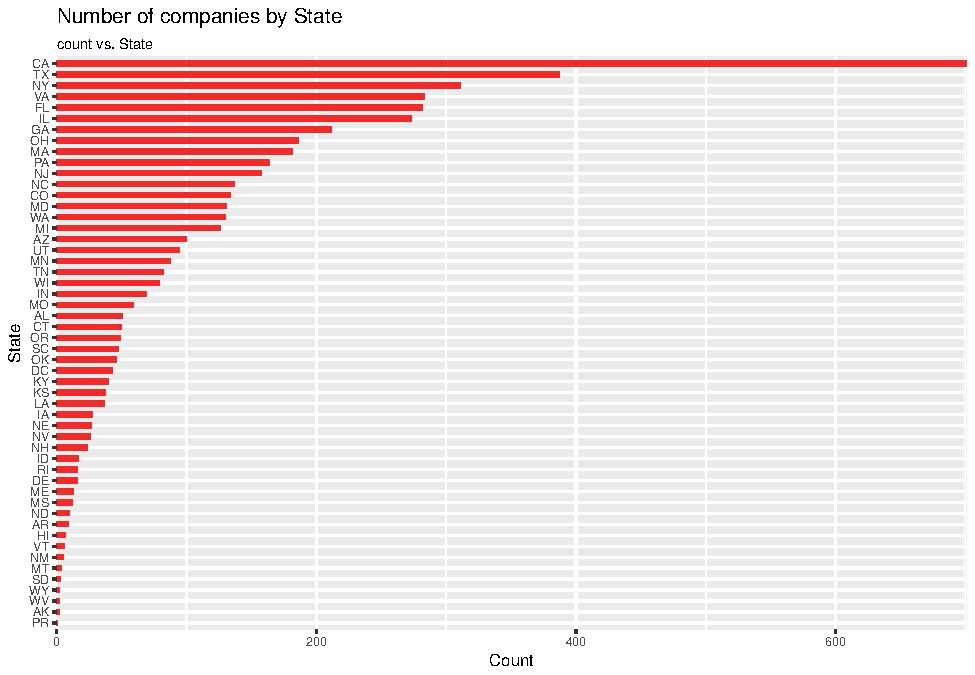
\includegraphics{DATA_608_Project_1_files/figure-latex/unnamed-chunk-5-1.pdf}

\subsection{Quesiton 2}\label{quesiton-2}

Lets dig in on the state with the 3rd most companies in the data set.
Imagine you work for the state and are interested in how many people are
employed by companies in different industries. Create a plot that shows
the average and/or median employment by industry for companies in this
state (only use cases with full data, use R's \texttt{complete.cases()}
function.) In addition to this, your graph should show how variable the
ranges are, and you should deal with outliers.

\begin{Shaded}
\begin{Highlighting}[]
\NormalTok{inc <-}\StringTok{ }\NormalTok{inc[}\KeywordTok{complete.cases}\NormalTok{(inc),]}

\NormalTok{find.third.state <-}\StringTok{ }\NormalTok{state.count }\OperatorTok
\StringTok{  }\KeywordTok{arrange}\NormalTok{(}\KeywordTok{desc}\NormalTok{(n))}
\NormalTok{find.third.state <-}\StringTok{ }\NormalTok{find.third.state}\OperatorTok{$}\NormalTok{State[[}\DecValTok{3}\NormalTok{]]}

\NormalTok{third.state <-}\StringTok{ }\KeywordTok{filter}\NormalTok{(inc, State }\OperatorTok{==}\StringTok{ }\NormalTok{find.third.state) }\OperatorTok
\StringTok{  }\KeywordTok{filter}\NormalTok{(}\KeywordTok{complete.cases}\NormalTok{(.))}

\NormalTok{third.state.table <-}\StringTok{ }\KeywordTok{group_by}\NormalTok{(third.state, Industry) }\OperatorTok
\StringTok{  }\KeywordTok{summarize}\NormalTok{(}\DataTypeTok{meanEmployment =} \KeywordTok{mean}\NormalTok{(Employees),}
            \DataTypeTok{medianEmployment =} \KeywordTok{median}\NormalTok{(Employees)}
\NormalTok{  ) }\OperatorTok
\StringTok{  }\KeywordTok{gather}\NormalTok{(property, count, meanEmployment, medianEmployment)}
\end{Highlighting}
\end{Shaded}

\begin{Shaded}
\begin{Highlighting}[]
\KeywordTok{ggplot}\NormalTok{(third.state.table, }\KeywordTok{aes}\NormalTok{(}\DataTypeTok{x=}\KeywordTok{reorder}\NormalTok{(Industry, count), }\DataTypeTok{y=}\NormalTok{count)) }\OperatorTok{+}
\StringTok{  }\KeywordTok{geom_bar}\NormalTok{(}\DataTypeTok{stat=}\StringTok{"identity"}\NormalTok{, }\DataTypeTok{position=}\StringTok{"dodge"}\NormalTok{, }\KeywordTok{aes}\NormalTok{(}\DataTypeTok{fill=}\NormalTok{property)) }\OperatorTok{+}
\StringTok{  }\KeywordTok{coord_flip}\NormalTok{() }\OperatorTok{+}
\StringTok{  }\KeywordTok{scale_fill_manual}\NormalTok{(}\DataTypeTok{values=}\KeywordTok{c}\NormalTok{(}\StringTok{"lightsteelblue4"}\NormalTok{, }\StringTok{"lightsteelblue2"}\NormalTok{), }\DataTypeTok{guide=}\KeywordTok{guide_legend}\NormalTok{(}\DataTypeTok{reverse=}\NormalTok{T)) }\OperatorTok{+}
\StringTok{  }\KeywordTok{scale_y_continuous}\NormalTok{(}\DataTypeTok{expand=}\KeywordTok{c}\NormalTok{(}\DecValTok{0}\NormalTok{,}\DecValTok{0}\NormalTok{))}
\end{Highlighting}
\end{Shaded}

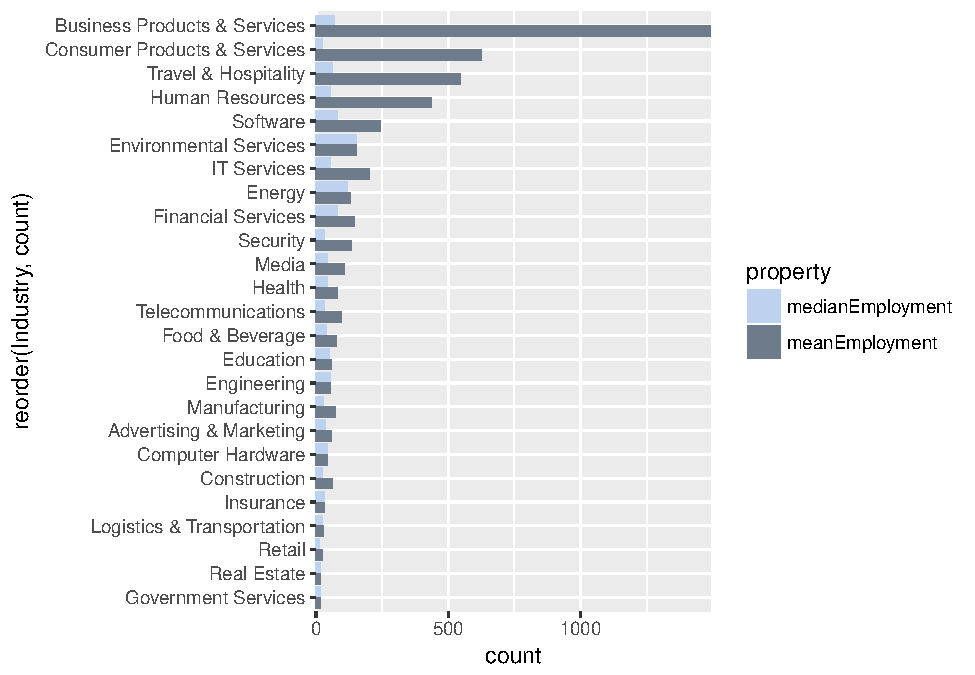
\includegraphics{DATA_608_Project_1_files/figure-latex/unnamed-chunk-7-1.pdf}

\texttt{Business\ Products\ \&\ Services} appears to be an outlier. If
we check the average difference between industry means, we can somewhat
regulate the outlier.

\begin{Shaded}
\begin{Highlighting}[]
\NormalTok{state.outlier <-}\StringTok{ }\NormalTok{third.state.table }\OperatorTok
\StringTok{  }\KeywordTok{filter}\NormalTok{(property }\OperatorTok{==}\StringTok{ "meanEmployment"}\NormalTok{)}
\NormalTok{state.outlier <-}\StringTok{ }\NormalTok{state.outlier[}\OperatorTok{-}\KeywordTok{c}\NormalTok{(}\DecValTok{2}\NormalTok{),] }\CommentTok{# drop the outlier}
\KeywordTok{mean}\NormalTok{(}\KeywordTok{diff}\NormalTok{(}\KeywordTok{sort}\NormalTok{(state.outlier}\OperatorTok{$}\NormalTok{count))) }\CommentTok{# calculate the average difference }
\end{Highlighting}
\end{Shaded}

\begin{verbatim}
## [1] 26.49105
\end{verbatim}

\begin{Shaded}
\begin{Highlighting}[]
\KeywordTok{max}\NormalTok{(}\KeywordTok{diff}\NormalTok{(}\KeywordTok{sort}\NormalTok{(state.outlier}\OperatorTok{$}\NormalTok{count)))}
\end{Highlighting}
\end{Shaded}

\begin{verbatim}
## [1] 191.6224
\end{verbatim}

We see the average difference between consecutive leading industries is
26.49105, with a max of 191.6224. With this in mind, I think we can cap
the outlier at \textasciitilde{}200 more than the second-highest.

\begin{Shaded}
\begin{Highlighting}[]
\NormalTok{third.state.edited <-}\StringTok{ }\NormalTok{third.state.table}
\NormalTok{third.state.edited[}\DecValTok{2}\NormalTok{,}\DecValTok{3}\NormalTok{] <-}\StringTok{ }\DecValTok{815}
\KeywordTok{ggplot}\NormalTok{(third.state.edited, }\KeywordTok{aes}\NormalTok{(}\DataTypeTok{x=}\KeywordTok{reorder}\NormalTok{(Industry, count), }\DataTypeTok{y=}\NormalTok{count)) }\OperatorTok{+}
\StringTok{  }\KeywordTok{geom_bar}\NormalTok{(}\DataTypeTok{stat=}\StringTok{"identity"}\NormalTok{, }\DataTypeTok{position=}\StringTok{"dodge"}\NormalTok{, }\KeywordTok{aes}\NormalTok{(}\DataTypeTok{fill=}\NormalTok{property)) }\OperatorTok{+}
\StringTok{  }\KeywordTok{coord_flip}\NormalTok{() }\OperatorTok{+}
\StringTok{  }\KeywordTok{scale_fill_manual}\NormalTok{(}\DataTypeTok{values=}\KeywordTok{c}\NormalTok{(}\StringTok{"lightsteelblue4"}\NormalTok{, }\StringTok{"lightsteelblue2"}\NormalTok{), }\DataTypeTok{guide=}\KeywordTok{guide_legend}\NormalTok{(}\DataTypeTok{reverse=}\NormalTok{T)) }\OperatorTok{+}
\StringTok{  }\KeywordTok{scale_y_continuous}\NormalTok{(}\DataTypeTok{expand=}\KeywordTok{c}\NormalTok{(}\DecValTok{0}\NormalTok{,}\DecValTok{0}\NormalTok{))}
\end{Highlighting}
\end{Shaded}

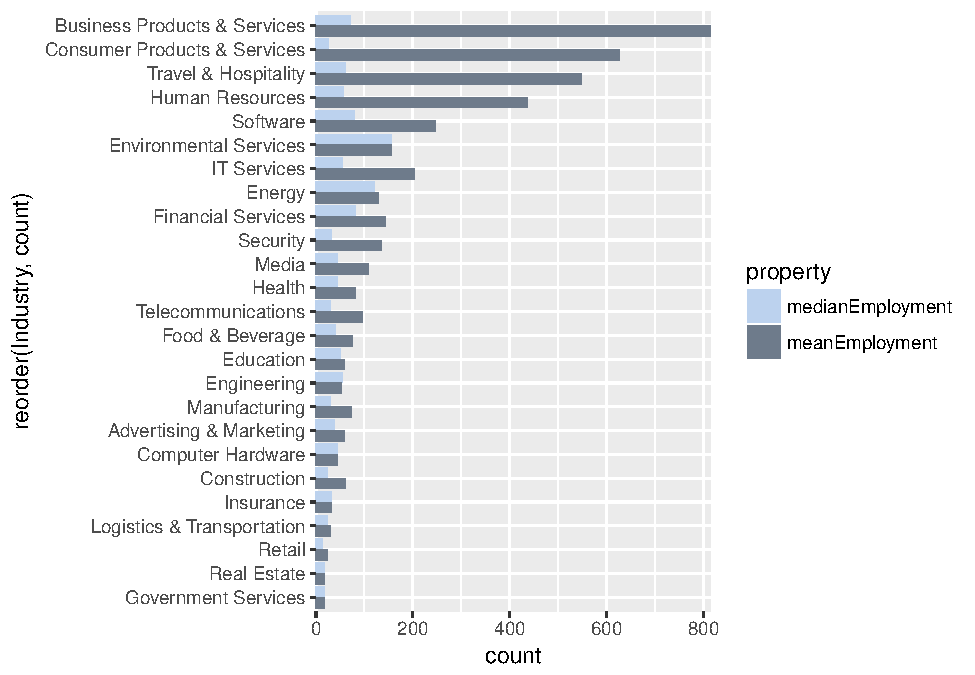
\includegraphics{DATA_608_Project_1_files/figure-latex/unnamed-chunk-9-1.pdf}

\subsection{Question 3}\label{question-3}

Now imagine you work for an investor and want to see which industries
generate the most revenue per employee. Create a chart that makes this
information clear. Once again, the distribution per industry should be
shown.

\begin{Shaded}
\begin{Highlighting}[]
\NormalTok{most.profitable <-}\StringTok{ }\NormalTok{inc }\OperatorTok
\StringTok{  }\KeywordTok{group_by}\NormalTok{(Industry) }\OperatorTok
\StringTok{  }\KeywordTok{summarize}\NormalTok{(}\DataTypeTok{rpe =} \KeywordTok{sum}\NormalTok{(Revenue)}\OperatorTok{/}\KeywordTok{sum}\NormalTok{(Employees))}
  
\KeywordTok{ggplot}\NormalTok{(most.profitable, }\KeywordTok{aes}\NormalTok{(}\DataTypeTok{x=}\KeywordTok{reorder}\NormalTok{(Industry, rpe), }\DataTypeTok{y=}\NormalTok{rpe)) }\OperatorTok{+}
\StringTok{  }\KeywordTok{geom_bar}\NormalTok{(}\DataTypeTok{stat=}\StringTok{"identity"}\NormalTok{, }\DataTypeTok{colour=}\StringTok{"slategrey"}\NormalTok{) }\OperatorTok{+}
\StringTok{  }\KeywordTok{coord_flip}\NormalTok{()}
\end{Highlighting}
\end{Shaded}

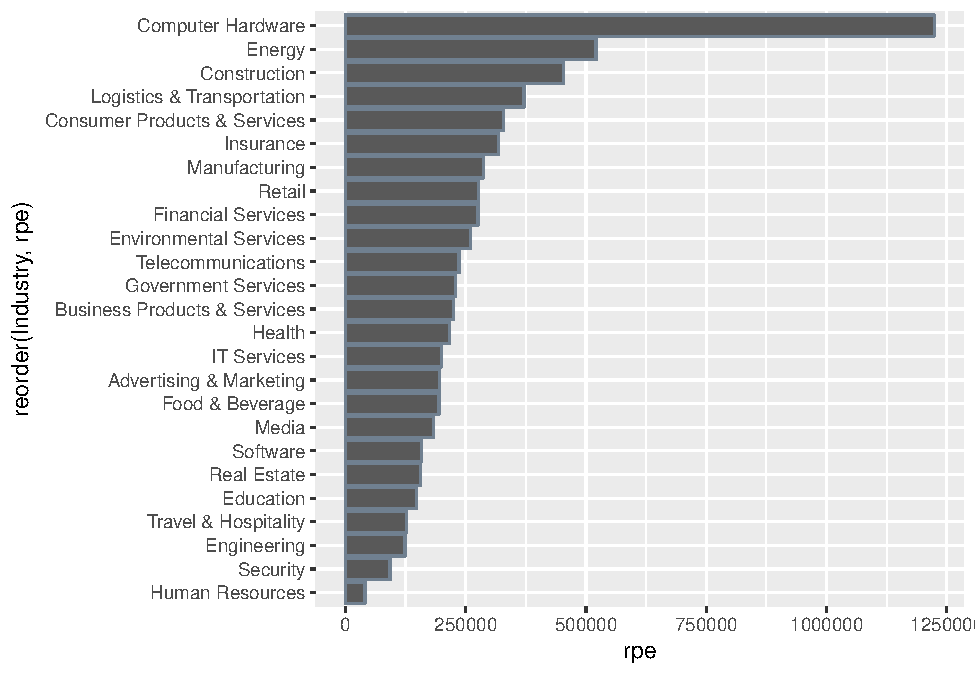
\includegraphics{DATA_608_Project_1_files/figure-latex/unnamed-chunk-10-1.pdf}

Once again, we have an outlier; in this case, it's
\texttt{Computer\ Hardware}. Using the same method as in problem 2,
we'll cap the outlier.

\begin{Shaded}
\begin{Highlighting}[]
\NormalTok{mp.edited <-}\StringTok{ }\NormalTok{most.profitable}
\KeywordTok{mean}\NormalTok{(}\KeywordTok{diff}\NormalTok{(}\KeywordTok{sort}\NormalTok{(mp.edited}\OperatorTok{$}\NormalTok{rpe)))}
\end{Highlighting}
\end{Shaded}

\begin{verbatim}
## [1] 49284.53
\end{verbatim}

\begin{Shaded}
\begin{Highlighting}[]
\KeywordTok{max}\NormalTok{(}\KeywordTok{diff}\NormalTok{(}\KeywordTok{sort}\NormalTok{(mp.edited}\OperatorTok{$}\NormalTok{rpe)))}
\end{Highlighting}
\end{Shaded}

\begin{verbatim}
## [1] 702642.5
\end{verbatim}

\begin{Shaded}
\begin{Highlighting}[]
\NormalTok{mp.edited[}\DecValTok{3}\NormalTok{,}\DecValTok{2}\NormalTok{] <-}\StringTok{ }\DecValTok{600000}

\KeywordTok{ggplot}\NormalTok{(mp.edited, }\KeywordTok{aes}\NormalTok{(}\DataTypeTok{x=}\KeywordTok{reorder}\NormalTok{(Industry, rpe), }\DataTypeTok{y=}\NormalTok{rpe)) }\OperatorTok{+}
\StringTok{  }\KeywordTok{geom_bar}\NormalTok{(}\DataTypeTok{stat=}\StringTok{"identity"}\NormalTok{, }\DataTypeTok{colour=}\StringTok{"slategrey"}\NormalTok{) }\OperatorTok{+}
\StringTok{  }\KeywordTok{coord_flip}\NormalTok{()}
\end{Highlighting}
\end{Shaded}

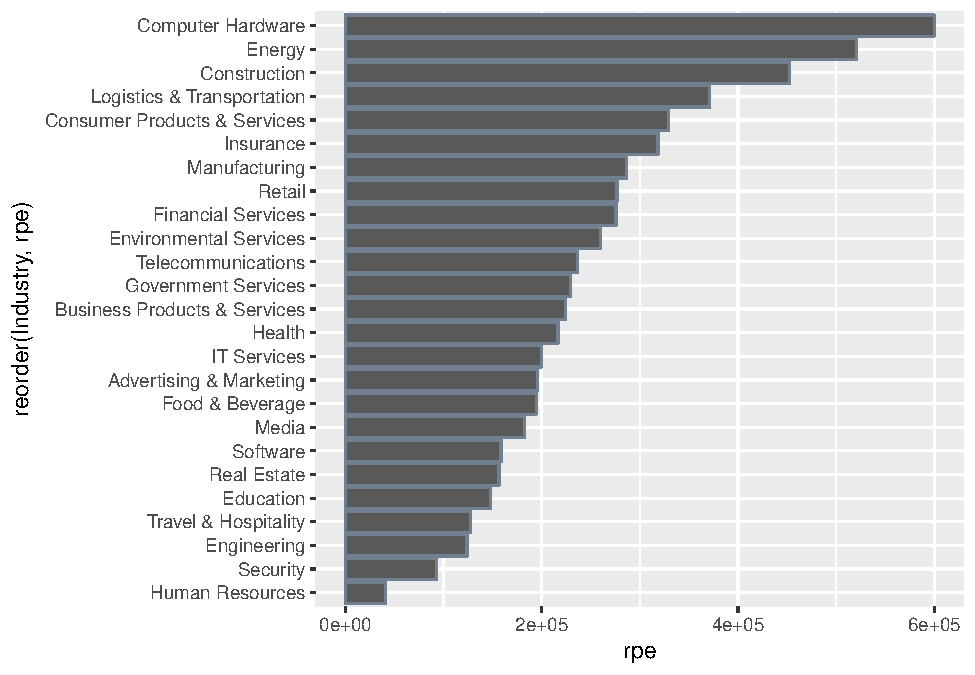
\includegraphics{DATA_608_Project_1_files/figure-latex/unnamed-chunk-11-1.pdf}


\end{document}
